\begin{figure}[t]
	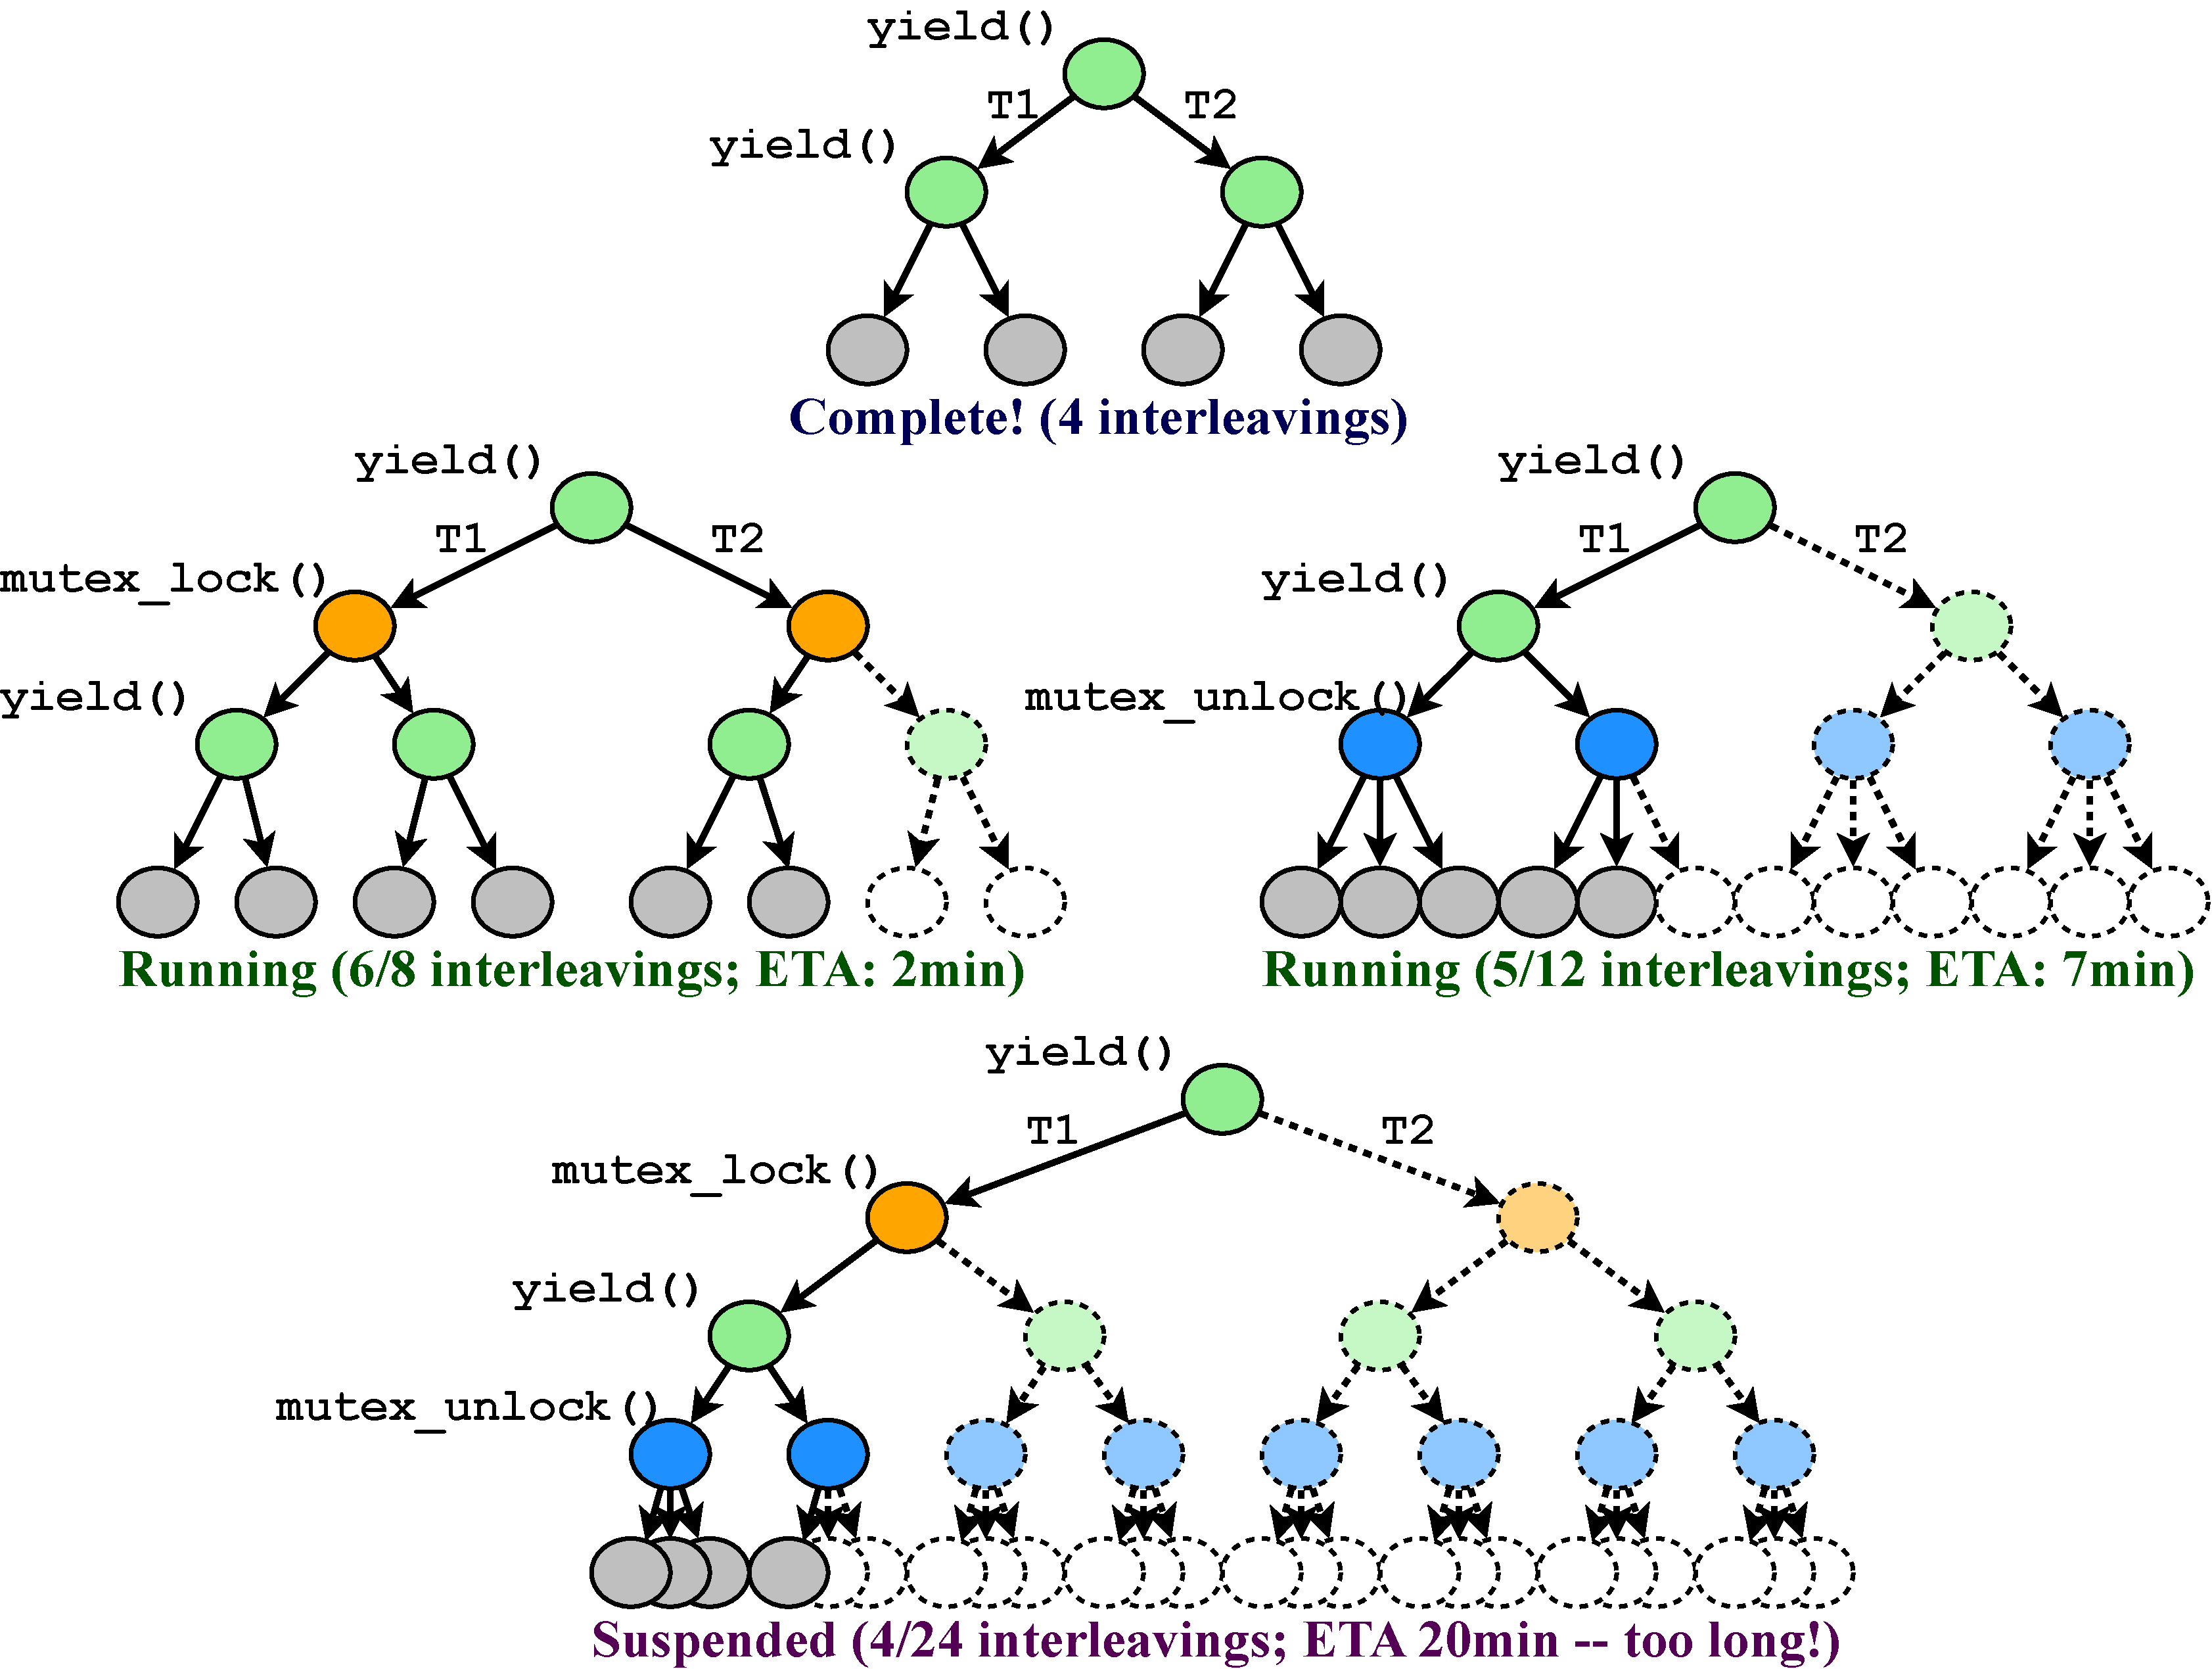
\includegraphics[width=0.48\textwidth]{trees.pdf}
	%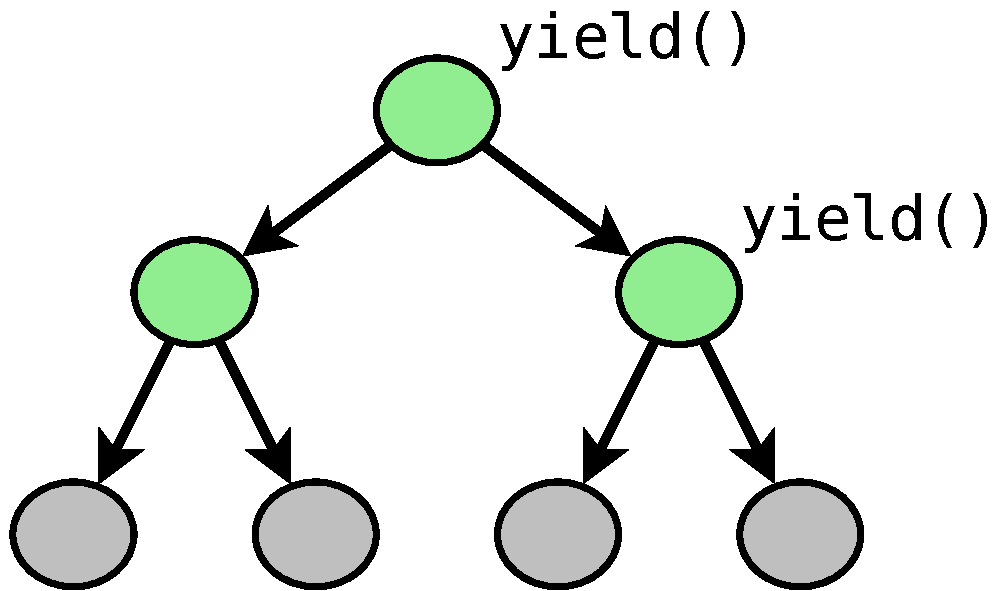
\includegraphics[width=0.15\textwidth]{tree0.pdf}
	%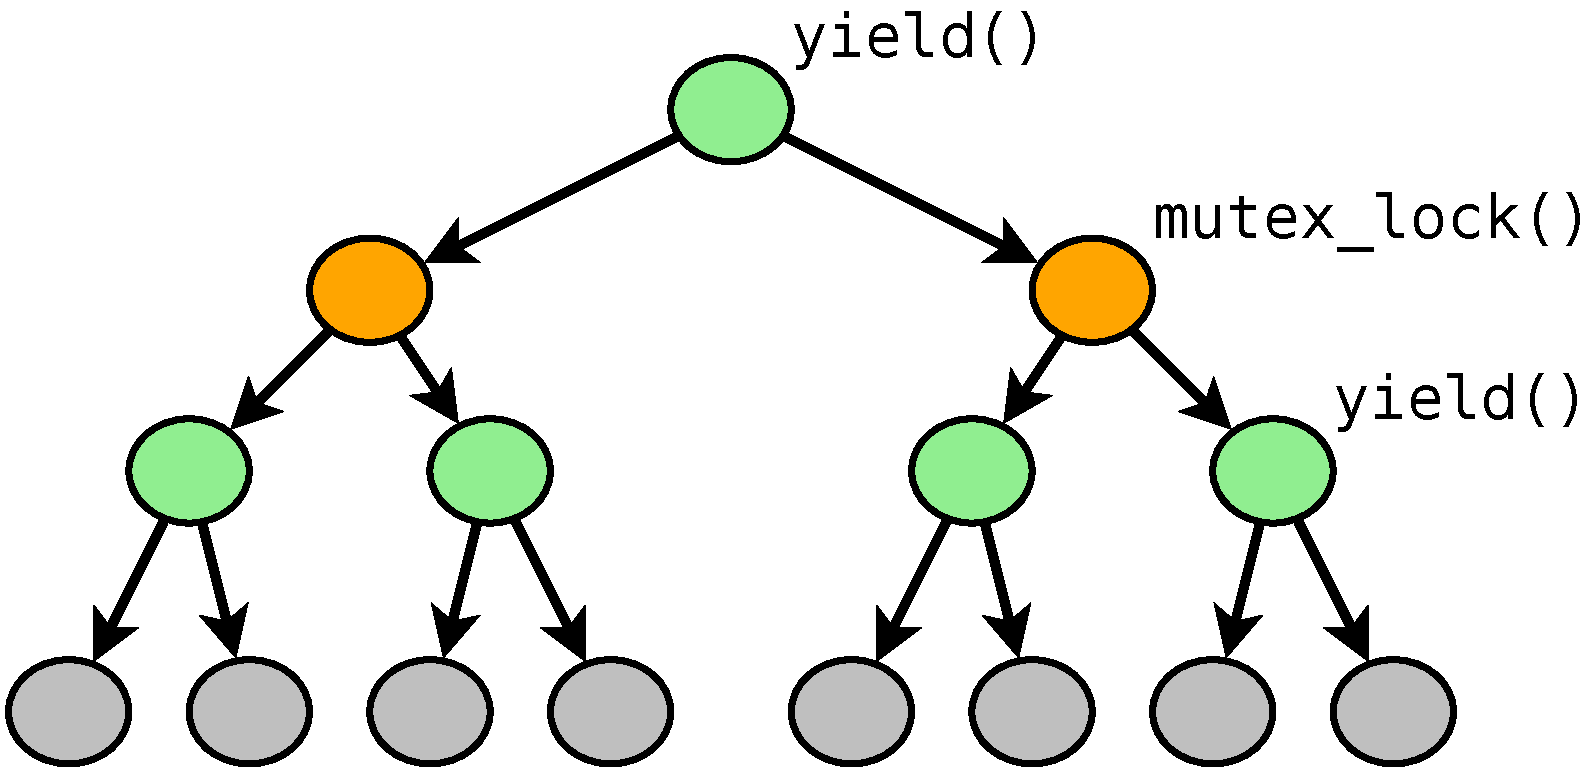
\includegraphics[width=0.225\textwidth]{tree1.pdf}
	%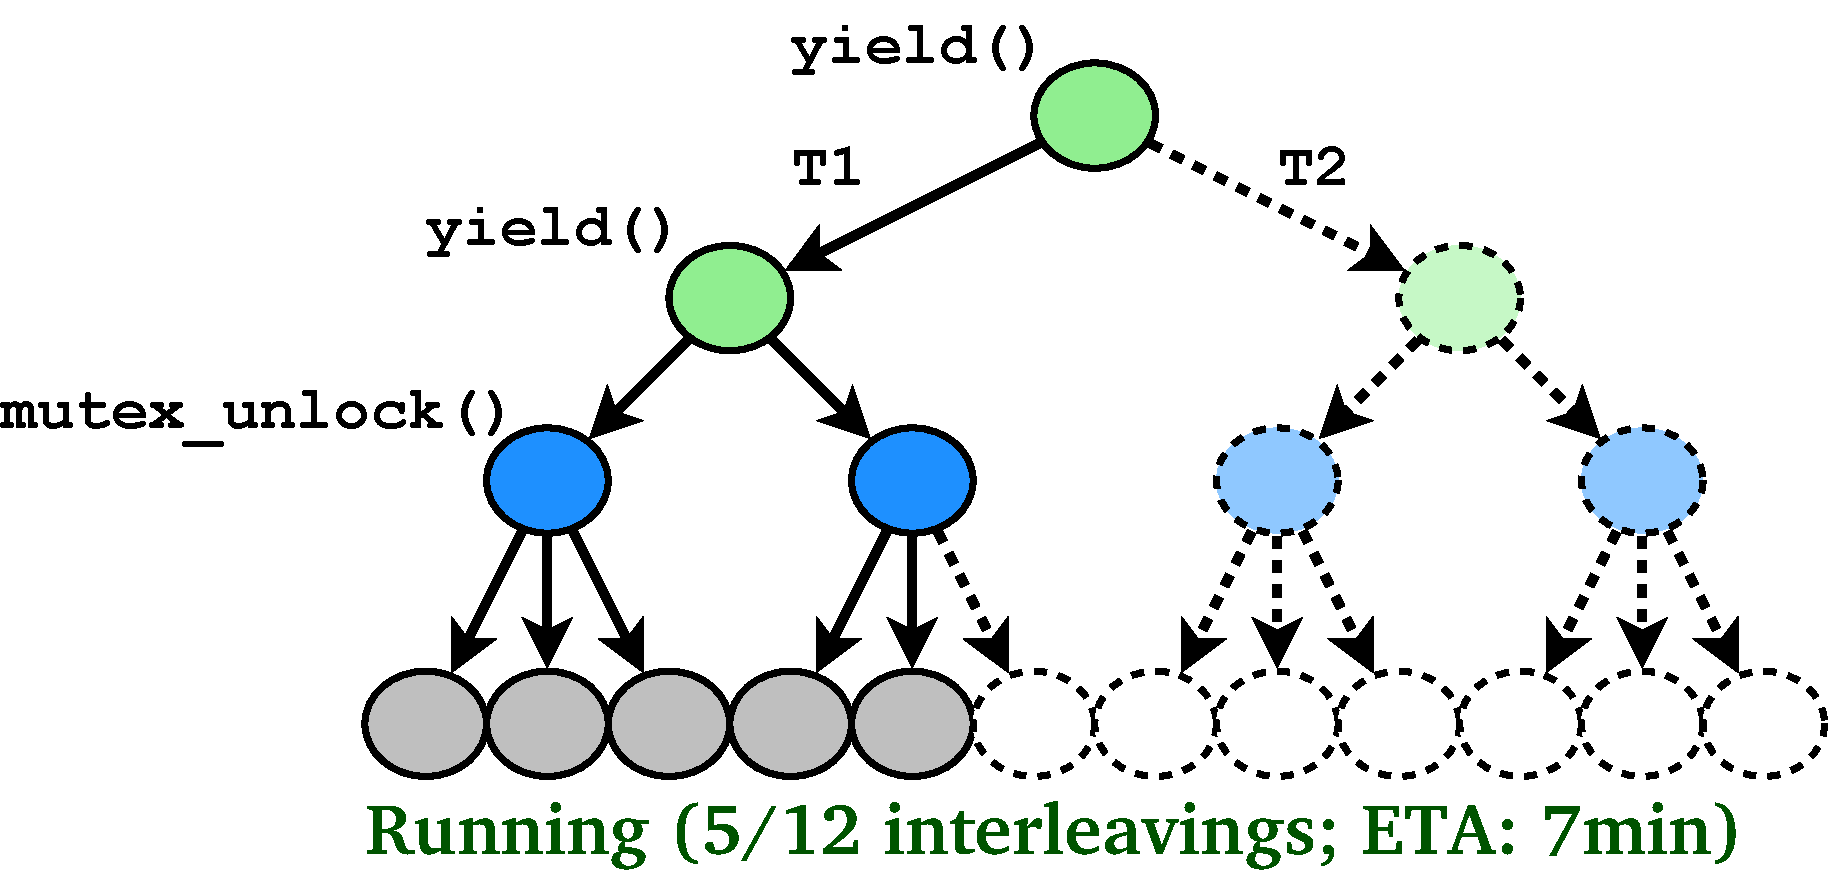
\includegraphics[width=0.25\textwidth]{tree2.pdf}
	%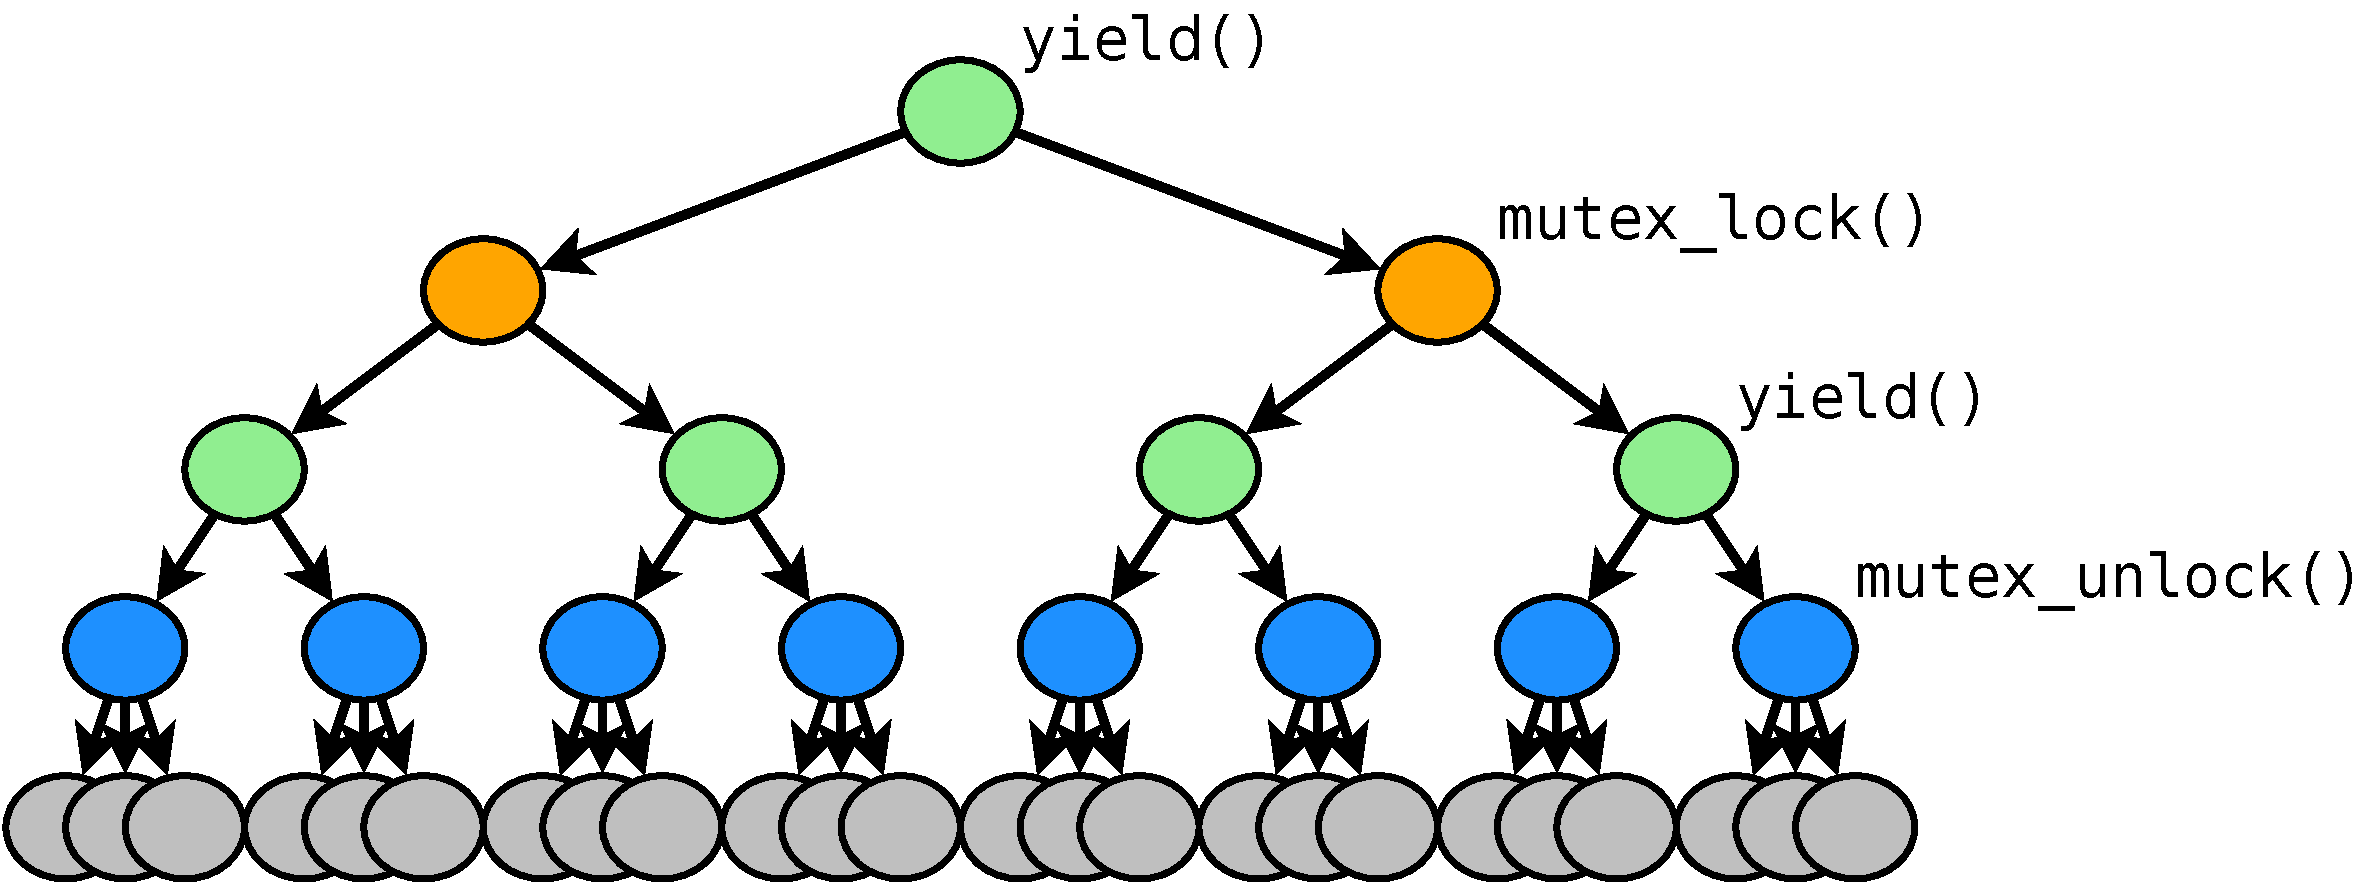
\includegraphics[width=0.35\textwidth]{tree3.pdf}
	\caption{Iterative Deepening example.
		The minimal state space (top) includes only voluntary thread switches, such as {\tt yield()} or {\tt cond\_wait()}.
		Multiple further tests can be run: preempting on calls to {\tt mutex\_lock} alone (left), {\tt mutex\_unlock} alone (right), or both together (bottom).
Each option increases the state space size by an unpredictable factor, so multiple state spaces should be tested in parallel.
Estimation techniques~\cite{estimation} inform which state spaces to prioritize.
}
	\label{fig:id}
\end{figure}
\section{Design}

Motivated by state-of-the-art tools' inflexibility to change their preemption points,
Iterative Deepening searches among different combinations of such points during a test,
deciding on-the-fly whether to pursue each resulting state space or abandon it in favour of smaller ones.
Different state spaces are generated based on {\em subsets} of the preemption points which prior work would use; for example, ``preempt on all calls to {\tt mutex\_lock} but not on {\tt mutex\_unlock}''.
We show a visualization in Figure~\ref{fig:id}.

Iterative Deepening depends heavily on state-space estimation \cite{estimation}
to understand which state spaces are likely to complete on time,
in advance of actually testing each interleaving within.
The purpose is to make decisions automatically about when to defer exploration of a state space,
so an inexpert user must provide only their total CPU budget as a test parameter,
and to enable completing appropriately-sized state spaces within that budget.

Note that Iterative Deepening is a {\em wrapper} algorithm around stateless model checking.
A model checking tool is still used to test each state space, and other reduction techniques are still applicable.
Moreover, because Iterative Deepening treats the set of preemption points as mutable,
it can add new ones reactively based on any runtime analysis.
In this paper we focus on dynamic data-race detection~\cite{tsan} as the mechanism for finding new preemption candidates.

\subsection{Terminology}

For the rest of the paper, we abbreviate {\em preemption point} (PP),
%For the remainder of the paper, we will abbreviate {\em preemption point} (PP),
{\em model checking} (MC),
{\em single-state-space model checking} (SSS-MC),% (i.e., the approach of prior work),
Dynamic Partial Order Reduction (DPOR), and {\em state space estimate} (ETA).

SSS-MC indicates the approach of prior model checking tools:
the set of PPs is fixed in advance, and the tool commits to testing every interleaving available via those PPs.
%Reduction techniques are often used to skip equivalent interleavings \cite{dpor}, and search-ordering strategies
Many techniques exist to skip equivalent interleavings and order the search to uncover bugs faster \cite{dpor,demeter,chess-icb,gambit},
but dynamic analysis cannot add new PPs or remove ineffective ones.

Please note the difference between data-race {\em candidates} and data-race {\em bugs}.
Because data-race analysis is prone to false-positives,
we classify unprotected access pairs separately from concrete observable failures, % "concrete"?
calling such pairs {\em data race candidates}.
Should a future interleaving, preempting during those accesses,
lead to a failure (e.g. assertion or deadlock), then we report a {\em data-race bug}.
Otherwise, if the access pair can be reordered, but does not produce a failure under any interleaving, it is a {\em benign data race}.
If they cannot be reordered at all, it is a {\em false positive}.
%TODO: Don't do this, below. Scan paper for uses of 'false positive' where you mean to say 'benign' or 'both'.
%For brevity, we count benign data races as a subset of false positives.

We also identify the {\em minimal} and {\em maximal state space} for each test.
The {\em minimal state space} includes only thread switches arising from normal execution (Figure~\ref{fig:id}).
The {\em maximal state space} is simply the one explored by SSS-MC: all statically-available PPs are enabled.
%However, should new data-race PPs be added during a test, the new maximal state space will be the one including those as well.
%% don't say this ^ -- because when you add dr pps, they add in pairs and there would be multiple maximals, at least until they each get explored and subseuqnetly add a pp of the other of the pair.

\subsection{Classifying data races as buggy or benign} % FIXME: dont say 'benign'; also, do you have enough left to say that this can even still be a full subsection?

\subsection{Choosing the best job}

% TODO: put colour in this code
\newcommand\PendingJobs{\ensuremath{\mathcal{P}}}
\newcommand\SuspendedJobs{\ensuremath{\mathcal{S}}}
\newcommand\GetETA[1]{ETA(#1)}
\newcommand\GetPPSet[1]{PPSet(#1)}
\begin{algorithm}[t]
	\SetKwInOut{Input}{Input}
	%\textbf{Function} GetBestJob($j_0$, PendingJobs, SuspendedJobs): \\
	\Input{$j_0$, the currently-running job}
	%\Input{$eta$, $j_0$'s predicted completion time}
	\Input{\PendingJobs, the list of pending jobs, sorted decreasingly by heuristic priority}
	\Input{\SuspendedJobs, the list of already-suspended jobs, sorted increasingly by ETA}
	\If{\GetETA{$j_0$} $<$ HeuristicETAFactor $\times$ TimeLeft()}{
		// Common case: Job is expected to complete. \\
		return $j_0$
	}
	\ForEach{job $j_P \in$ \PendingJobs}{
		// Don't run a pending job if a subset of it is already suspended; its ETA would be at least as bad. \\
		\If {$\forall j_S \in$ \SuspendedJobs, \GetPPSet{$j_S$} $\not\subset$ \GetPPSet{$j_P$}}{
			return $j_P$
		}
	}
	%// no pending jobs; maybe resume a suspended job \\
	\ForEach{job $j_S \in$ \SuspendedJobs}{
		\If{\GetPPSet{$j_0$} $\not\subset$ \GetPPSet{$j_S$}
			$\land$
			\GetETA{$j_0$} $>$ \GetETA{$j_S$}}{
			// If a subset of $j_S$ is also suspended, don't run the larger one first. \\
			\If{$\forall j_{S2} \in$ \SuspendedJobs, \GetPPSet{$j_{S2}$} $\not\subset$ \GetPPSet{$j_S$}}{
				return $j_S$
			}
		}
	}
	// $j_0$'s ETA was bad, but nothing else was better. \\
	return $j_0$
	\caption{Suspending exploration of a state space in favour of a potentially smaller one.}
	\label{alg:shouldworkblock}
\end{algorithm}

With a limited CPU budget, we must avoid running tests that are likely to time out.
When a MC instance reports an ETA too high,
we compare other yet-untested PP sets to find another job more likely to complete in time.
Our method for doing so, listed in Algorithm~\ref{alg:shouldworkblock}, is the heart of Iterative Deepening\footnote{
Though its worst-case performance is $O(mn)$ in the
%number of pending and suspended jobs,
sizes of $\mathcal{P}$ and $\mathcal{S}$,
in practice the non-constant portion beyond line 4 runs very infrequently
and is negligible compared to the exponentially-sized state spaces.}.
Its main feature is understanding that if \GetPPSet{$j_1$} $\subset$ \GetPPSet{$j_2$},
and $j_1$ is suspended,
then $j_2$'s state space is guaranteed to be strictly larger, so $j_2$ will take at least as long.
Hence we should avoid testing $j_2$ unless $j_1$'s ETA improves over time.
%reveals that it might finish in time after all.
Similarly, when some job finds a bug, we cancel all pending superset jobs, as they would find the same bug.

%
We also account for the inherent inaccuracy of ETA estimates.
Line 1 heuristically scales up the time remaining to avoid suspending jobs too aggressively
in case their ETAs are actually overestimated.
Lines 12-14 account for the
%bizarre
possibility that among two suspended jobs,
%given two jobs,
%%$j_1,j_2$,
\GetPPSet{$j_1$} $\subset$ \GetPPSet{$j_2$}
but
\GetETA{$j_1$} $>$ \GetETA{$j_2$}.
This can arise because estimates tend to get more accurate over time,
and $j_1$ perhaps ran much longer before suspending.
% In such scenarios,
We heuristically assume the smaller job's ETA is more accurate
to avoid repeatedly resuming larger jobs briefly while their ETAs only become worse
(it lets us avoid thrashing in \quicksand).

%%%%%%%%%%%%%%%%%%%%%%%%%%%%%%%%%%%%%%%%%%%%%%%%%%%%%%%%%%%%%%%%%%%%%%%%%%%%%%%%

\section{Implementation}

\subsection{Landslide}
\label{sec:landslide}

We chose \landslide~\cite{landslide} as our stateless model checker due to its ability to trace program execution at the granularity of individual instructions and memory accesses, which dynamic data-race detection requires.
\landslide~implements DPOR,
%\cite{dpor},
state space estimation, and a hybrid lockset/happens-before data-race analysis.
% TODO: \cite{fairstatelessmc} instead or in addition?
It avoids state space cycles (e.g. ad-hoc synchronization with {\tt yield()} or even {\tt xchg} loops) with a heuristic similar to Fair-Bounded Search \cite{bpor}. % TODO: devote a paragraph to this, after talking about drs in locks
% this line can be cut if space is needed
It can test both user-level and kernel-level code, although is limited to timer-driven nondeterminism.
Its bug-detection metrics include assertion failure, deadlock, segfault, heap checking (like Valgrind~\cite{valgrind}), and a heuristic infinite loop/livelock check.

{\bf Restricting PPs with stack trace predicates.}
Most MCs preempt indiscriminately on any sync API call, regardless of the call-site.
However, when testing a particular module in a large codebase,
the user is likely uninterested in PPs arising from other modules.
\landslide~provides the {\tt within\_function} configuration command for a user to identify which call-sites matter most.
Before inserting a PP, \landslide~requires at least one argument to {\tt within\_function} to appear in the current thread's stack trace.
%The {\tt without\_function} directive works similarly, but as a blacklist.
The {\tt without\_function} directive is the dual of {\tt within\_function}, indicating a blacklist.
Multiple invocations can be used; later ones take precedence.
%\cite{landslide} provides further detail on this feature.

{\bf Data races in lock implementations.}
Data race tools in prior work \cite{tsan,portend} recognize the implementations of sync primitives to avoid spuriously flagging memory accesses resulting from the lock implementation itself.
Assuming the locks are already correct enables productive data-race analysis on the rest of the codebase.
With testing limited to one execution, even if you wished to test for lock bugs, data-race analysis would still uselessly flag every single access pair in the lock implementation, requiring human attention to verify.
However, Iterative Deepening can automatically verify a large quantity of data-race candidates as benign.
Hence, we extended \landslide~with a custom option to change the lock-set tracking to include accesses from {\tt mutex\_lock()} and {\tt mutex\_unlock()} in the analysis. (Accesses from other sync functions, such as {\tt cond\_wait()}, would either be included already, or be protected by an internal mutex.)
% TODO: Add a code sample showing how the lockset boundaries change? If there's room?

\subsection{Quicksand}

\quicksand~is an independent program that wraps the execution of several \landslide~instances.
The implementation is roughly 3000 lines of C.
It uses a thread pool to schedule the available state spaces,
sorting such jobs according to their status among a running queue, pending queue, and suspended queue.
Jobs are further prioritized by number of PPs, ETA, and whether they include data-race PPs.

{\bf Initial PPs.}
For testing user-space code, we seed the exploration with the four subsets of ``hard-coded'' locking API PPs shown in Figure~\ref{fig:id}.
By extension, these also introduce preemptions on any other sync primitives implemented with mutexes,
such as condvars, semaphores, and r/w locks.
Preempting on voluntary switches such as {\tt yield} is necessary for the invariant that only one thread runs between consecutive PPs,
so the {\tt yield} PP is always implicitly enabled.

For kernel-level testing, we consider interrupt-disabling to be analogous to locking,
so (e.g. on x86) we also preempt just before {\tt cli} and just after {\tt sti}\footnote{
During data-race detection, {\tt cli}/{\tt sti} are treated as a single global lock,
as {\tt cli}'d memory accesses can still race with others that have interrupts on.}.
% FIXME: "What happened to yield?" "Yield is implicitly included in each subset."
\quicksand~is configured to begin with the subsets
$\{ \}$,
$\{lock\}$,
$\{unlock\}$,
$\{cli\}$,
$\{sti\}$,
and $\{lock,unlock,cli,sti\}$.
As a heuristic, we don't bother with every intermediate subset such as $\{lock,sti\}$,
which could potentially be improved in future work (\sect{\ref{sec:future}}).

{\bf Communication protocol.}
The interface to \landslide~, which any similar MC could implement, has two parts.
First, when starting each job, \quicksand~creates a configuration file declaring which PPs to use,
% can lose this line due to space
among other options such as mutex-testing mode,
passed as an argument to \landslide.
Then, a dedicated \quicksand~thread communicates with the \landslide~process via message-passing.%on a FIFO pipe.
\landslide~messages \quicksand~after testing each new interleaving to report updated progress and ETA,
whenever a new data-race candidate is found, and whenever a bug is found.
\quicksand~in turn replies whether the test should suspend/resume due to too high ETA, or quit due to timeout.

{\bf Heuristics.}
% List of all heuristix:
% HOMESTRETCH - last 60sec of test, don't suspend
% ETA_THRESH - "to let its ETA stabilize"
% eta factor
% shold_reproduce -- small dr jobs are not allowed to add further instances of themself (why not? don't remember)
% priority change between suspected and confirmed dr
Algorithm~\ref{alg:shouldworkblock} allows heuristically scaling a job's ETA when comparing to the time budget,
to express how optimistic we are about the estimate's accuracy.
We use 2 as this scaling factor based on the results in \cite{estimation},
though we allow changing it via the command line.
We also include a heuristic to
%ignore ETAs entirely
never suspend jobs before they pass a certain threshold of interleavings tested,
for which we choose 32,
so their ETAs have some time to stabilize.

We classify data-race candidates as {\em single-order} or {\em both-order} \cite{portend}
based on whether \landslide~observed the access pair ordered one or both ways while testing the original state space,
Single-order candidates are much more likely to be false-positives
(though we cannot say for sure before preempting during the access itself, hence the heuristic),
so we prioritize jobs with both-order data-race PPs.
For single-order races, we do not add PPs for the later access at all;
should they be needed, preempting on the first access will suffice to upgrade it to both-order.

% If there's room, mention the cant_swap mechanism for killing the top half of deferred jobs.

\subsection{Data-race preemption points}

When \landslide~detects a data race, it reports each of the two memory accesses involved in the race.
Each report indicates the program counter value (PC) associated with the access, as well as some further conditions to help filter away unrelated executions of the same instruction on different data.
(For example, many parts of a codebase might call {\tt list\_insert()}, but only one callsite does so without adequate locking.)
Ideally, the PC would be qualified by a full backtrace, but tracing the stack is too expensive to do for each shared memory access.
Instead, \landslide~qualifies the PC with
(a) the current thread ID and
% FIXME: We don't actually do this.
(b) the most recent {\tt call} instruction.
% (a crude approximation of a stack trace)
% which are much cheaper, as we carry them around all the time already
Note that we do {\em not} qualify data races by the shared memory address,
which can change based on different interleavings of previous code
(for example, depending on the result of {\tt malloc()}).
% especially when malloc is involved.
%Figure~\ref{fig:dont-filter-dr-by-address} shows example code where qualifying by memory address will miss the bug.


When \quicksand~receives a data race report, it adds two new jobs to its workqueue:
a ``small'' job to preempt on the racing instruction only,
and a ``big'' job to preempt on that instruction as well as each PP used by the reporting job.
%
Hence each {\em pair} of racing accesses will spawn four new jobs, as shown in Figure~\ref{fig:new-dr-jobs}.
Rather than adding a maximal job with both new PPs at once, we prefer to add smaller jobs which have a higher chance of completing in time.
If those state spaces are bug-free, they will in turn add the maximal job later.
%
The rationale of spawning multiple jobs is that which will be more fruitful cannot be known in advance:
while the big job risks not completing in time,
the small job risks missing the data race entirely if the original PPs were required to expose it.
In practice, we observed some bugs found quickly by these small jobs, and other bugs missed by the small jobs found eventually by the big jobs,
which motivates the need for Iterative Deepening to decide at runtime which jobs to prioritize.
% TODO: Put numbers here.

\begin{figure}[t]
	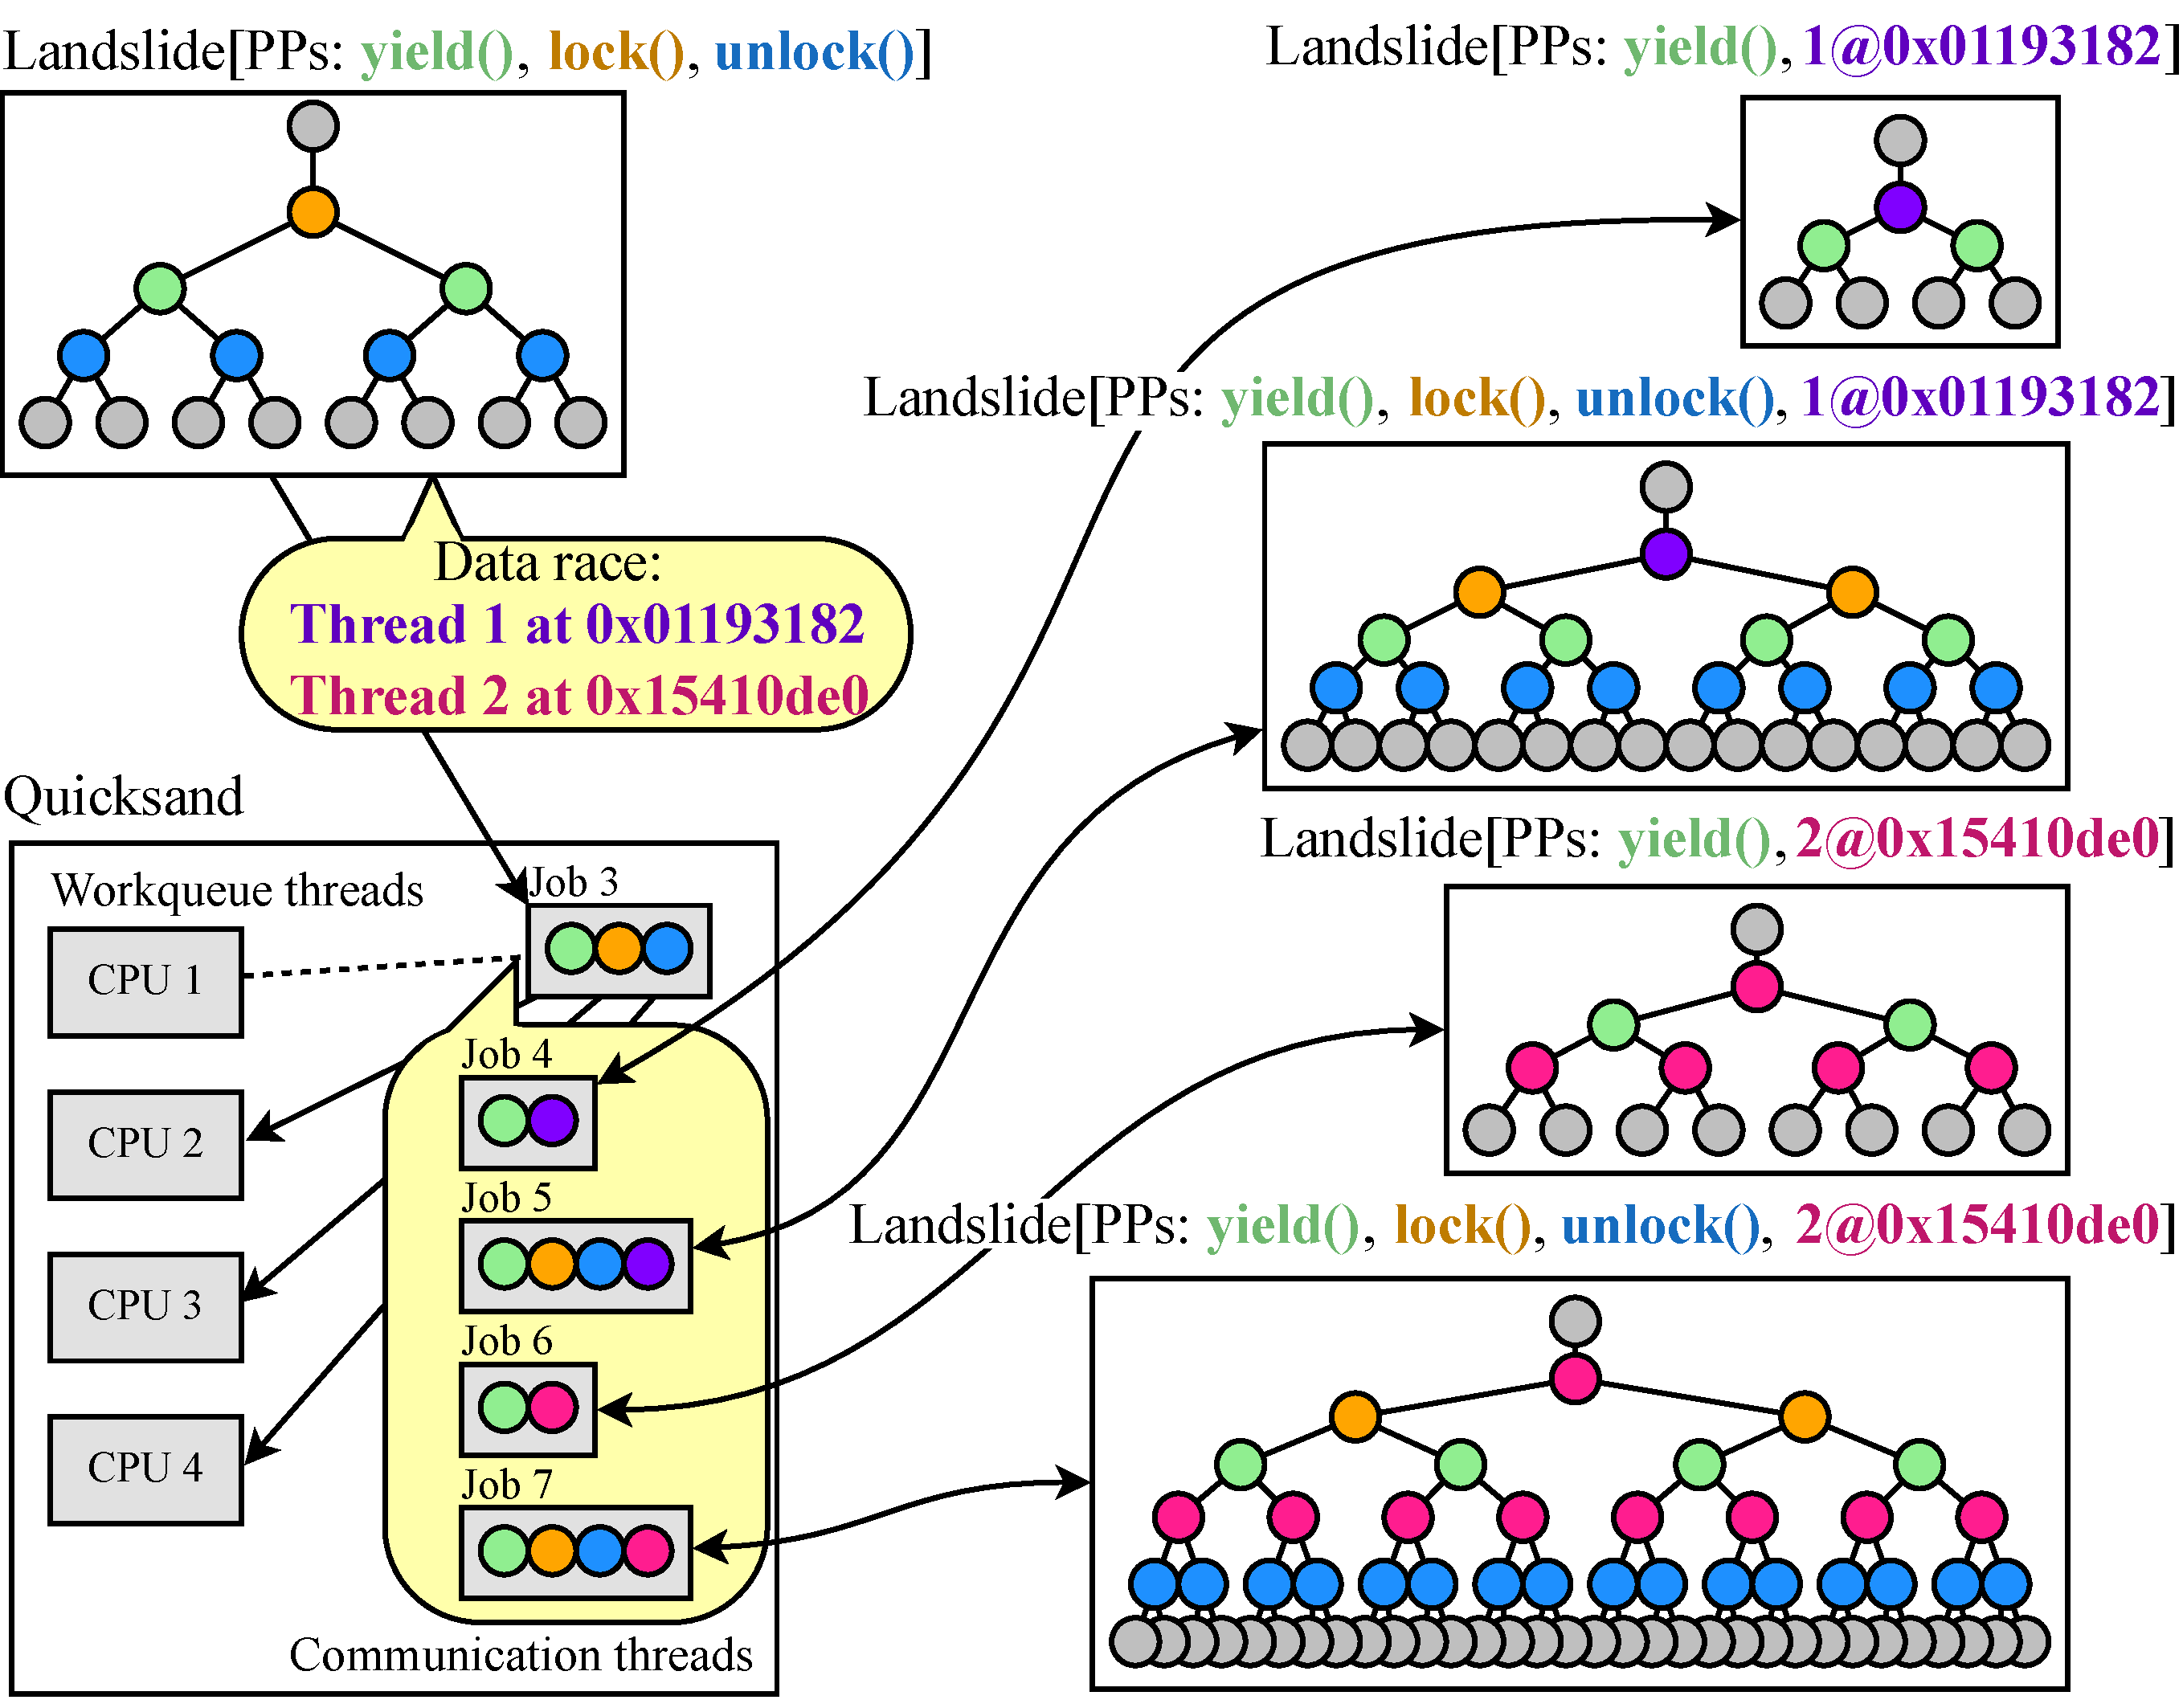
\includegraphics[width=0.48\textwidth]{dr-jobs.pdf}
	\caption{\quicksand~manages the exploration of multiple state spaces, communicating with each MC instance to receive ETAs, data race candidates, and bug reports.
		When an access pair is reported as a data race, we generate a new PP for each access and add new jobs corresponding to different combinations of those with the existing PPs.}
	\label{fig:new-dr-jobs}
\end{figure}

\subsection{Suppressing ``malloc-recycle'' false positives}
\label{sec:recycle}

% TODO: Understand what prior work means by 'happens before'. It's different from our MUST happen before relation.
% TODO: Understand how it relates to this. Would it scoop us? Or are we outside their model?

We identify a particular class of false positive data-race candidate in which the associated memory is recycled by {\tt malloc} between the two accesses.
Figure~\ref{fig:recycle} shows a common code pattern and interleaving which can expose such behavior.
If the {\tt malloc} on line 4 returns the same address passed to {\tt free} on line 2, then lines 1 and 7 will be flagged as a data race.
We term this a {\em malloc-recycle data race}.
To the human eye, this is obviously a false positive: reordering lines 4-7 before lines 1-2 will change {\tt malloc}'s return value, causing {\tt x} and {\tt y} to no longer collide.
Here, Thread 2's logic usually corresponds to the initialization pattern \cite{eraser}, but for generality we have added a {\tt publish} action on line 6.

\begin{figure}[t]
	\small
\begin{tabular}{rll}
	& \multicolumn{2}{c}{\texttt{struct x \{ int foo; int baz; \} *x;}} \\
	& \multicolumn{2}{c}{\texttt{struct y \{ int bar; \} *y;~~~~~~~~~~}} \\
	\\
	& Thread 1 & Thread 2 \\
	1 & \texttt{\hilight{brickred}{x->foo = ...;}} & \\
	2 & \texttt{\hilight{olivegreen}{free}(x);} \\
	3 & & \texttt{// x's memory recycled} \\
	4 & & \texttt{y~=~\hilight{olivegreen}{malloc}(sizeof *y);} \\
	5 & & \texttt{// ...initialize...}\\
	6 & & \texttt{publish(y);} \\
	7 & & \texttt{\hilight{brickred}{y->bar = ...;}} \\
\end{tabular}
\caption{A common execution pattern with {\tt malloc()} that produces false positive data race candidates.}
\label{fig:recycle}
\end{figure}

% This class of false positive is unique to heap-allocated memory, among all ways threads could communicate. By contrast, global memory has unlimited lifetime, and message-passing primitives enforce a must-happens-before relationship which precludes the race.

It is quite simple to mechanically recognize when {\tt x} and {\tt y} correspond to different abstract allocations despite colliding on address.
We implemented this check by adding a generation counter to \landslide's heap tracking:
each allocation is given a unique ID,
and when evaluating whether two heap accesses can race,
the IDs of their containing blocks must match.
However, when limited to a single execution, suppressing any data race matching this pattern is unsound.
Consider the more unusual program in Figure~\ref{fig:recycle-bug}:
Now, the memory is recycled the same way, but the racing access's address is not tied to {\tt malloc}'s return value.
Hence, reordering lines 6-7 before line 3 will cause {\tt x} and {\tt x2} to race.

\begin{figure}[t]
	\small
\begin{tabular}{rll}
	& Thread 1 & Thread 2 \\
	1 & \texttt{publish(x);} & \\
	2 & \texttt{\hilight{brickred}{x->foo = ...;}} & \\
	3 & \texttt{\hilight{olivegreen}{free}(x);} \\
	4 & & \texttt{x2 = get\_published\_x();} \\
	5 & & \texttt{// x's memory recycled} \\
	6 & & \texttt{y~=~\hilight{olivegreen}{malloc}(sizeof *y);} \\
	7 & & \texttt{\hilight{brickred}{x2->foo = ...;}} \\
\end{tabular}
\caption{If a single-pass data race detector discarded candidates matching the malloc-recycle pattern,
it would miss the bug in this adversarial program.}
\label{fig:recycle-bug}
\end{figure}

%Because concurrent {\tt malloc} is often implemented with an internal lock, under a {\em pure} happens-before analysis,
Note that under a {\em pure happens-before} analysis,
these accesses are not considered concurrent % at all
because of {\tt malloc}'s internal locking events,
and would not result in such false positives.
However, pure happens-before can miss many real bugs \cite{hybriddatarace,tsan},
so in our context it is more appropriate to use the
{\em limited happens-before} relation in a hybrid approach with lockset tracking.
%the hybrid approach combining lockset tracking and the {\em limited} happens-before relation is not vulnerable to false negatives,

Fortunately, when data-race detection is combined with DPOR and Iterative Deepening, pruning these false positives is sound even when such adversarial programs are considered.
This makes it unnecessary to verify such data races by actively adding more preemptions,
achieving a potentially combinatorial reduction in how many state spaces we generate.
%Intuitively, we need not worry about cases such as Figure~\ref{fig:recycle-bug} because,
%should they be true races,
%DPOR will reorder threads sufficiently for the malloc-recycle pattern to disappear.
We provide a proof sketch below.

\renewcommand\proofname{Proof Sketch}

\begin{theorem}[Soundness of eliminating malloc-recycle races]
If a malloc-recycle data race is not a false positive,
%DPOR will reorder threads such that
DPOR will test an alternate thread interleaving in which
%either
the accesses still race without fitting the malloc-recycle pattern.
%, or a use-after-free bug will be reported immediately.
\end{theorem}

\begin{proof}
By definition of the malloc-recycle pattern,
any such program must contain an access {\tt x1} by one thread T1,
followed by a {\tt free} and a {\tt malloc} possibly by either thread,
followed by an access {\tt x2} by the other thread T2. % not depending on the result of the middle malloc.
For brevity we say that T1 performs the {\tt free} and T2 the subsequent {\tt malloc}; the other cases are similar.
We also assume the only way for the program to get pointers to heap memory is through {\tt malloc};
hence, there must also be some ``publish'' action {\tt p} by T1 which communicates the address to T2.
Because this is a true data race, {\tt p} must occur before {\tt x1}, as {\tt x2} cannot be reordered before {\tt p}.

We now show that a PP will be identified during T1 between {\tt p} and {\tt x1}.
The publish action must involve some thread communication, whether through a shared data structure or message-passing API.
If locking or message-passing is used, our set of hard-coded PPs suffices.
Otherwise, {\tt p} (and the corresponding read by T2) will be a data race, although it may itself be a malloc-recycle race.
In this case we use induction on the pointer chain leading to {\tt x}:
in the base case, {\tt p} is global or obtained via message-passing,
and in the inductive step, DPOR will reorder threads sufficiently to identify the PP on {\tt p}.
Hence there will be a PP between {\tt p} and {\tt x1} no matter the mode of communication.

By definition of DPOR, this PP causes {\tt x2} to be reordered before {\tt x1} while not changing {\tt x2}'s location.
As T2's {\tt malloc} now occurs before T1's {\tt free}, it will allocate different memory.
Hence {\tt x1} and {\tt x2} will be in the same allocation;
hence the accesses can race without fitting the malloc-recycle pattern.
% Mario-man is very very hunger from not having enough plumming jobs, so his Quest for Eat and Dollars.
% This spells QED so we are done.
\end{proof}

Note especially that our reasoning does not require PPs on the internal locking of {\tt malloc} or {\tt free},
which are ideal candidates to ignore via {\tt without\_function} (\sect{\ref{sec:landslide}}) to reduce state space size.
Our full proof
{\em [submitted as supplementary material; will be cited as a tech report in the final version of the paper]}
discusses our assumptions explicitly and provides the similar cases in more detail.
\renewcommand\proofname{Proof}

%For further discussion and for the full proof, refer to
%{\em our supplementary material which we will cite as a tech report in the final version of the paper}.
